\chapter{Early Visual System}
\label{chap:visual_system}
This thesis focuses on modeling the \emph{primary visual cortex} (V1), a
critical structure in the early stages of visual processing in the mammalian
brain. V1 has been extensively studied for decades (\citet{hubel1965receptive}) 
and has served as a central subject
in both experimental and computational neuroscience. In this chapter, we
provide an overview of the components most relevant to our work, while
omitting a comprehensive review of the entire system. For a more detailed
examination, readers may refer to standard neuroscience texts such as
\citet{bear2020neuroscience} or \citet{goebel2004visual} which served
us as a source of information for the majority of this section.

\section{Neuron}
\label{sec:neuron}
The fundamental unit of neural processing in the brain is \emph{neuron}, a highly
specialized cell designed for the reception, integration, and transmission of
electrochemical signals. Neurons are different from other cell types due to their
unique morphology and functional properties, which allow for rapid and complex information
processing. The basic structure of a neuron comprises three principal components:

\begin{description}
    \item[Soma (Cell Body):] The \emph{soma} contains the nucleus and the essential 
    organelles required for protein synthesis, metabolic regulation, and general 
    neuronal maintenance. It plays a crucial role in the integration of synaptic 
    inputs received by the dendrites.

    \item[Dendrites:] The \emph{dendrites} emerge from the soma and serve as the 
    primary sites to receive synaptic input from other neurons.
    Their extensive arborization increases the surface area for synaptic connections, 
    allowing the integration of thousands of excitatory and inhibitory signals.

    \item[Axon:] The \emph{axon} is a specialized elongated part responsible 
    for transmitting electrical impulses over long distances to target neurons. 
    It originates at \emph{axon hillock}, a critical site for the initiation of the 
    action potential, and ends at \emph{axon terminals}, where synaptic communication 
    occurs.
\end{description}

The detailed anatomy of a neuron is illustrated in Figure \ref{fig:neuron}.

\begin{figure}
    \centering
    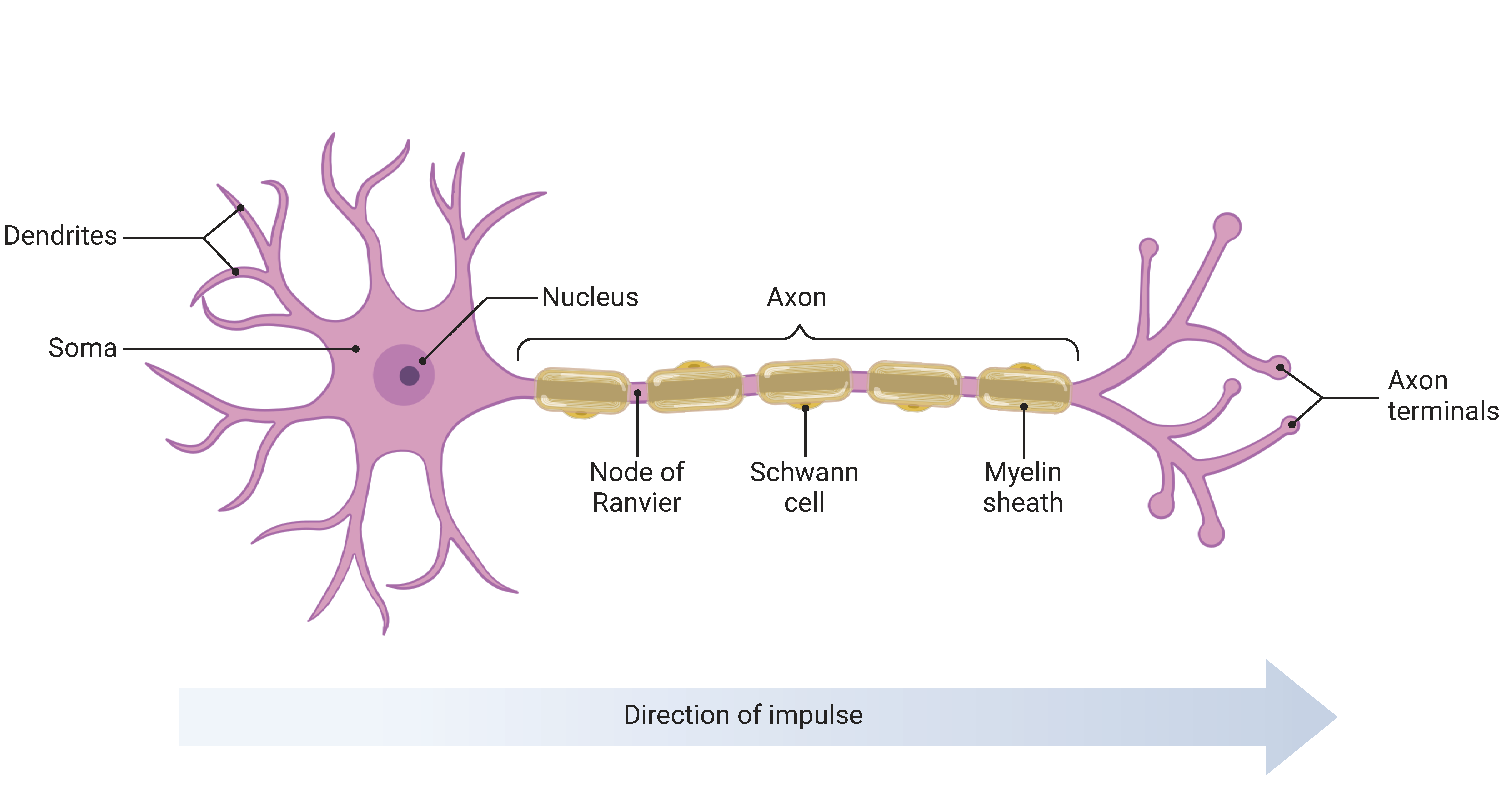
\includegraphics[width=\linewidth]{img/neuron_anatomy.pdf}
    \caption{\textbf{Neuron Anatomy} Illustration of a neuron anatomy. 
    "Created in BioRender. Beinhauer, D. (2025) https://BioRender.com/m351rlh "}
    \label{fig:neuron}
\end{figure}


\subsection{Axon Overview}
\label{subsec:axon}

The axon is uniquely adapted for efficient signal propagation, facilitated by specialized
ion channels and a range of structural proteins. At its terminal, the axon contains
synaptic vesicles, membrane-bound structures that store \emph{neurotransmitters}, chemical messengers
essential for synaptic communication. Upon arrival of an action potential, these vesicles
undergo exocytosis, releasing neurotransmitters into the synaptic cleft to influence the
activity of the postsynaptic neuron. Common neurotransmitters include glutamate (the main excitatory neurotransmitter in the central nervous system), 
gamma-aminobutyric acid (GABA) (the main inhibitory neurotransmitter),
as well as glycine and acetylcholine, which play critical roles in both central and
peripheral neural circuits.

\subsection{Action Potential}
\label{subsec:action_potential}
The primary mechanism by which neurons communicate is \emph{action potential}, a rapid, 
all-or-nothing electrical signal that propagates along the axon. This process is governed
by differences in ion concentration gradients across the neuronal membrane and the resulting
electrical potential differences.

At rest, neurons maintain a resting membrane potential of approximately $-65 \text{mV}$, a
state established by selective ion permeability and the activity of the sodium-potassium 
($\text{Na}^{+}/\text{K}^{+}$) pump. This pump actively transports $\text{Na}^{+}$ ions 
out of the cell and $\text{K}^{+}$ 
ions into the cell, maintaining concentration gradients essential for neuronal excitability. Other
key ions, such as chloride ($\text{Cl}^{-}$) and calcium ($\text{Ca}^{2+}$), also contribute to membrane dynamics, 
with their extracellular concentrations exceeding intracellular levels, except for $\text{K}^{+}$, which
is more concentrated within the neuron. A substantial portion of the brain's energy
consumption is dedicated to preserving these ionic gradients.

The action potential follows a well-defined sequence of events that are also illustrated in the Figure \ref{fig:action_potential}. The steps are the following:

\begin{enumerate}
    \item \textbf{Generator Potential and Threshold Activation:} Synaptic inputs induce localized changes in membrane potential, termed generator potentials. If sufficient excitatory input depolarizes the membrane to a threshold potential, typically around $-55 \text{mV}$, an action potential is triggered.
    \item \textbf{Rising Phase and Depolarization:} Voltage-gated $\text{Na}^{+}$ channels open, allowing $\text{Na}^{+}$ 
    ions to enter the neuron. This influx further depolarizes the membrane, causing a rapid shift toward positive values.
    The combined effects of the electrical gradient and the $\text{Na}^{+}$ concentration gradient drive this process, culminating in a phase known as the overshoot, where the membrane potential momentarily becomes positive.
    \item \textbf{Falling Phase and Repolarization:} As depolarization peaks, voltage-gated $\text{K}^{+}$ channels 
    open while $\text{Na}^{+}$ channels undergo inactivation. The efflux of $\text{K}^{+}$ ions restores the negative membrane potential, marking the beginning of repolarization.
    \item \textbf{Undershoot and Hyperpolarization:} $\text{K}^{+}$ conductance temporarily exceeds resting levels, causing the membrane potential to drop below the original resting value. This undershoot ensures that the neuron does not immediately refire.
    \item \textbf{Refractory Periods:}
    \begin{enumerate}
        \item \textbf{Absolute Refractory Period:} During this phase, $\text{Na}^{+}$ channels remain inactivated, preventing any 
        new action potential from occurring.
        \item \textbf{Relative Refractory Period:} The membrane is still hyperpolarized, requiring a stronger than normal depolarization to initiate a new action potential.
    \end{enumerate}
\end{enumerate}

\begin{figure}
    \centering
    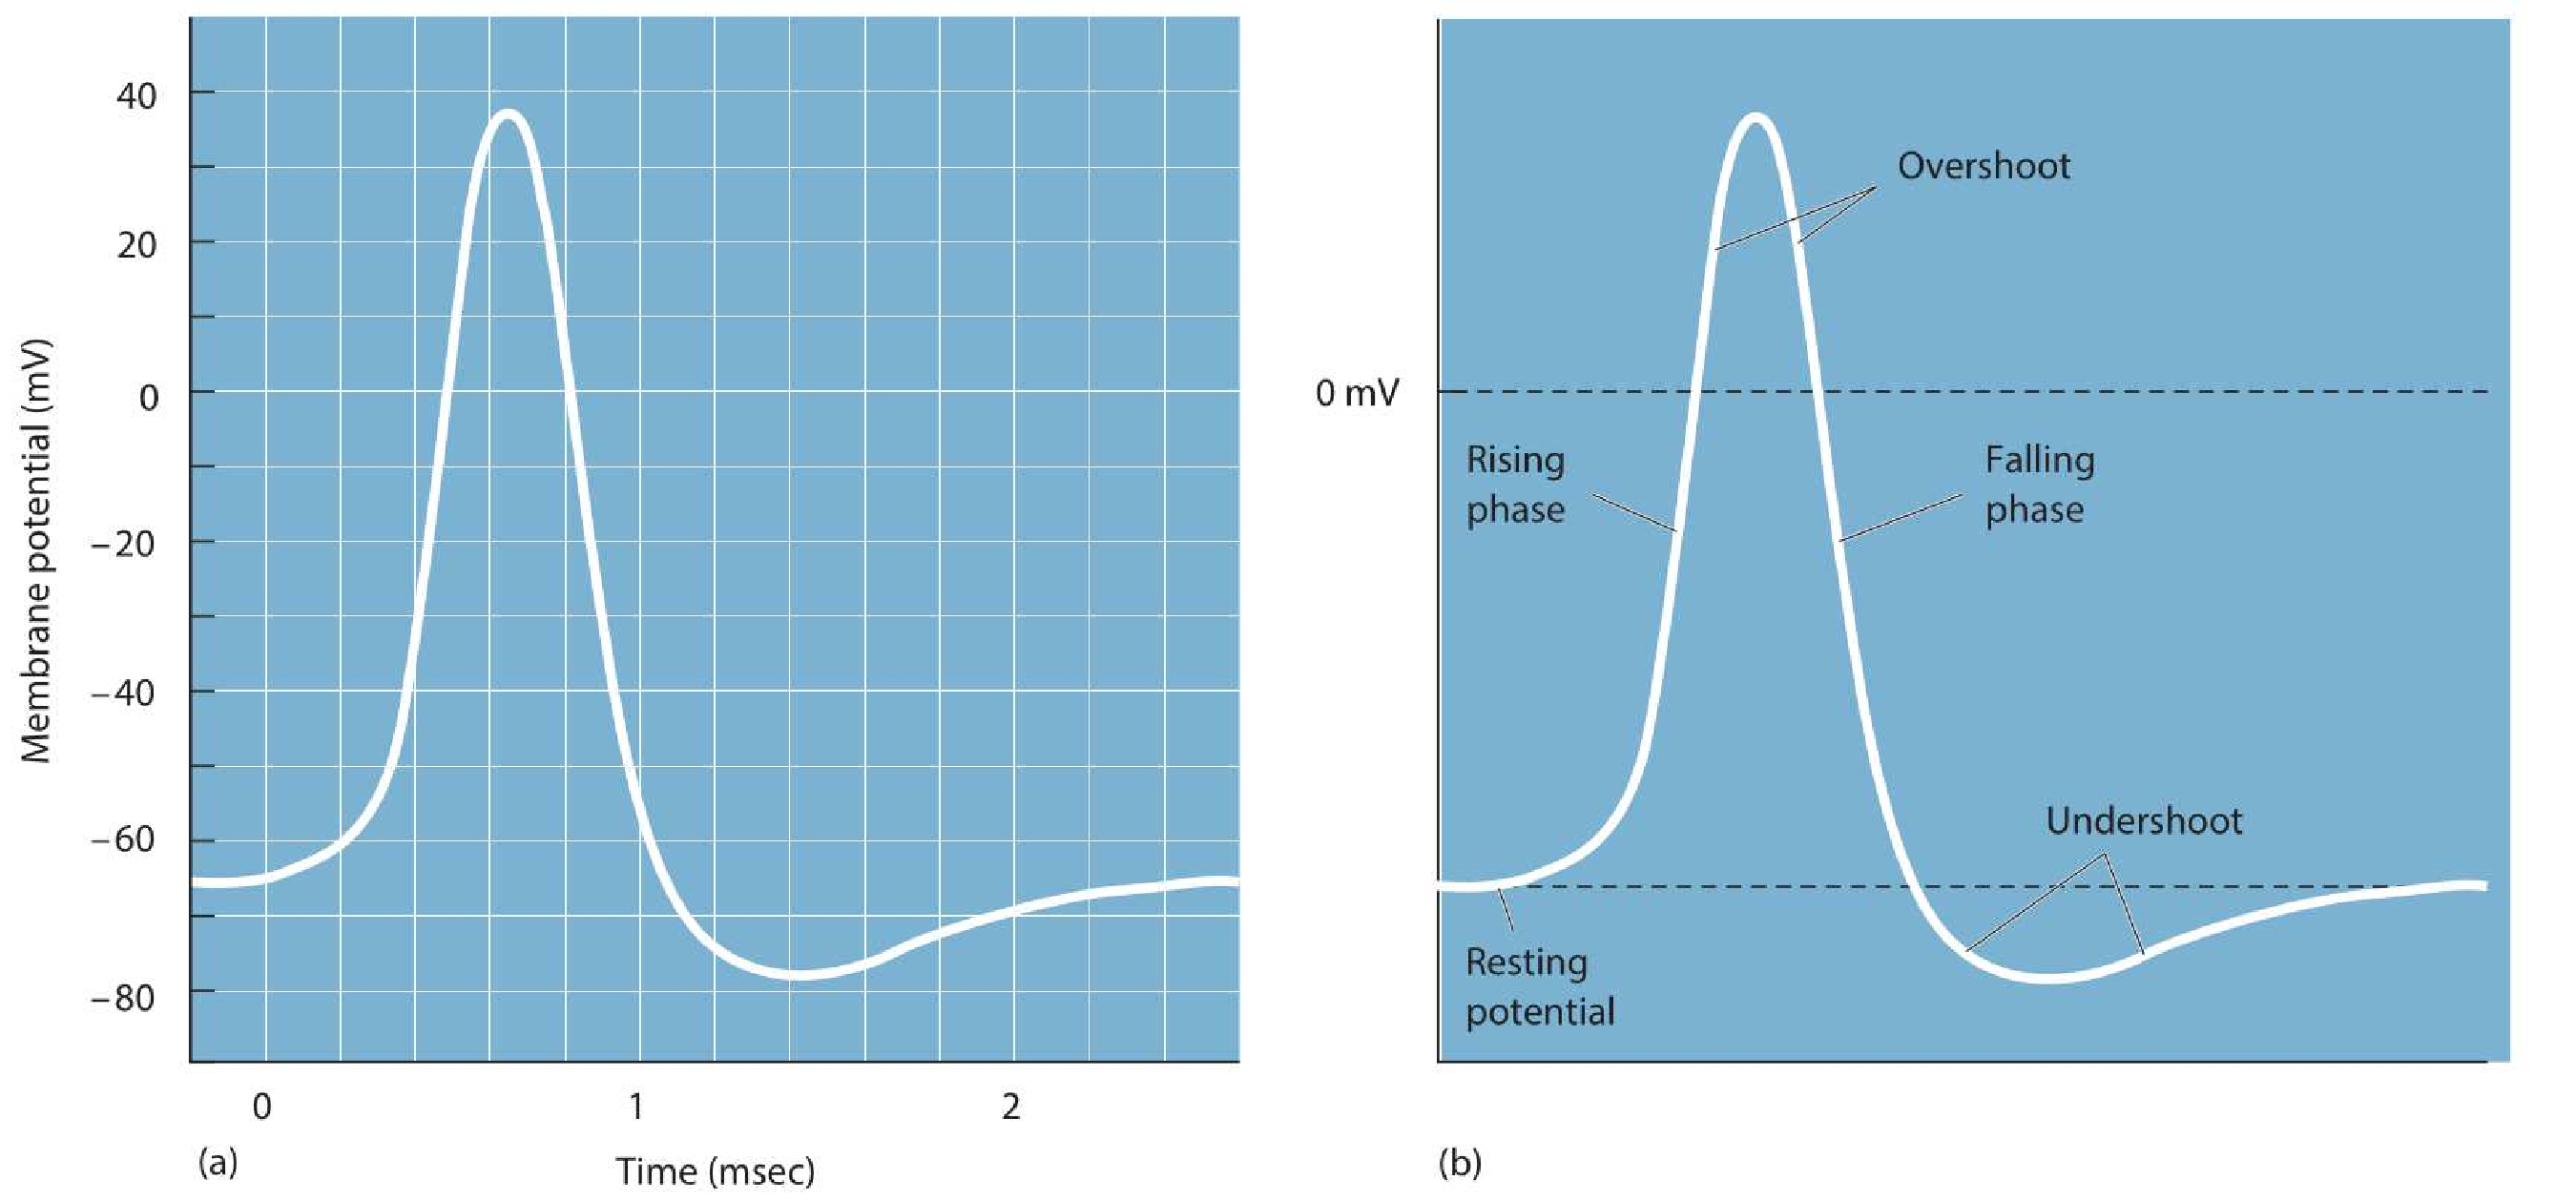
\includegraphics[width=\linewidth]{img/action_potential.pdf}
    \caption{\textbf{An action potential} \textbf{a)} An action potential displayed by an oscilloscope. \textbf{b)} The parts of an action potential. The figure and the labels are taken from \emph{Neuroscience} (\citet{bear2020neuroscience} (3rd Edition), p. 77).}
    \label{fig:action_potential}
\end{figure}

This directional propagation of the action potential, typically from the soma to the axon terminal, is ensured
by the sequential opening and inactivation of ion channels along the axon.

\subsection{Axonal Conduction and Myelination}
\label{subsec:axonal_conduction}
Efficient conduction of action potentials over long distances is critical for
rapid neural communication. The speed of propagation is significantly enhanced by
myelination, a process in which oligodendrocytes (in the central nervous system) 
and Schwann cells (in the peripheral nervous system) wrap axons in layers of myelin, 
a lipid-rich insulating substance. Myelin sheaths function to reduce ion leakage and
increase conduction velocity through saltatory conduction. Instead of propagating
continuously along the axon, action potentials "jump" between gaps in the myelin, 
known as the \emph{nodes of Ranvier}, where voltage-gated ion channels are concentrated. 
This results in dramatically increased signal transmission speeds, particularly
in long-range axons. This intricate structure is also depicted in Figure \ref{fig:neuron}.

\subsection{Synaptic Transmission}
\label{subsec:synaptic_transmission}
At the synaptic terminal, neurotransmitters stored in synaptic vesicles are released
in response to the action potentials arriving. This process, known as synaptic transmission,
involves the following steps:

\begin{enumerate}
    \item \textbf{Calcium Influx:} The arrival of an action potential opens voltage-gated 
    $\text{Ca}^{2+}$ channels, allowing $\text{Ca}^{2+}$ ions to enter the axon terminal.
    \item \textbf{Vesicle Fusion and Neurotransmitter Release:} Elevated intracellular $\text{Ca}^{2+}$ levels trigger neurotransmitter exocytosis.
    \item \textbf{Receptor Activation:} Neurotransmitters diffuse across the synaptic cleft and bind to receptors in the postsynaptic neuron, modulating its membrane potential. 
\end{enumerate}

Based on their effects on the postsynaptic membrane, synaptic connections can be classified as follows.
\begin{description}
    \item[Excitatory synapses:] These facilitate depolarization of the postsynaptic neuron, increasing the likelihood of generation of action potentials.
    \item[Inhibitory synapses:] These hyperpolarize the postsynaptic membrane, reducing the probability of an action potential.
\end{description}

This delicate balance between excitatory and inhibitory signaling is fundamental to neural circuit function and regulates processes such as sensory perception, cognition, and motor control.

\section{General Structure of the Early Visual System}
\label{sec:general_structure}
A significant portion of the human brain, nearly half, is dedicated to visual processing. 
The initial stage of this process occurs in the so-called \emph{Early Visual System}.

Visual signals travel in the form of light, passing through the complex optical
system of the eye and then projected onto the retina. The retina, a thin layer of neural tissue, 
is responsible for detecting light and performing initial signal processing. From there, 
the signal is transmitted through the optic nerve to the optic chiasm, where the visual information
is split based on the visual field. The signal then continues through the optic tract
to the \emph{Lateral Geniculate Nucleus} (LGN) of the thalamus. The LGN plays a crucial role
in the early stages of visual processing, refining the signal before transferring the
majority to \emph{primary visual cortex} (V1) via optical radiation. 
V1 is the first cortical area fully dedicated to visual processing, where more complex
computations take place. Once the signal exits V1, it is relayed to higher-order visual
areas responsible for advanced visual interpretation and processing.

\section{Eye}
\label{sec:eye}
One of the primary functions of the eye is to capture electromagnetic signals from
the environment, modulate them using its intricate optical system, and project them
onto the retina. The eye consists of multiple specialized structures that
appropriately bend and focus light. For a detailed anatomical description, 
refer to Figure \ref{fig:eye} and the relevant literature such as \citet{snell2013clinical}.

\begin{figure}
    \centering
    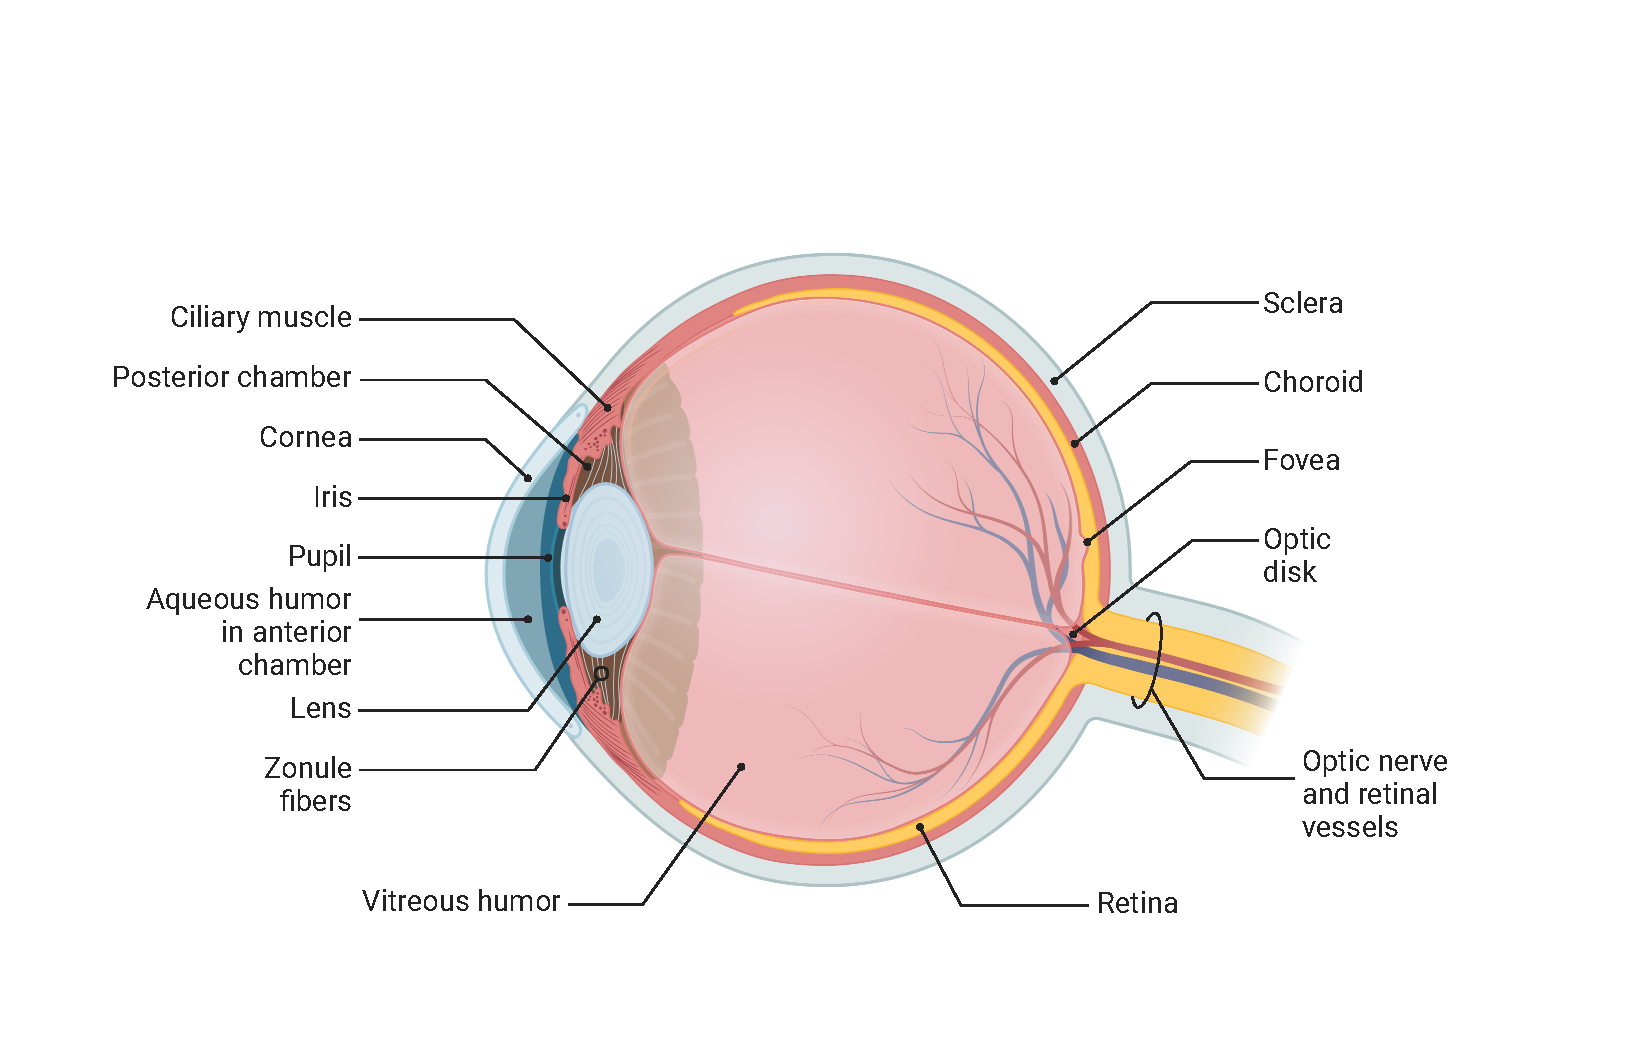
\includegraphics[width=\linewidth]{img/eye.pdf}
    \caption{\textbf{An anatomy of an eye} An illustration of an eye anatomy. Based on \citet{bear2020neuroscience} (3rd Edition), p. 283. "Created in BioRender. Beinhauer, D. (2025) https://BioRender.com/8n8epge".}
    \label{fig:eye}
\end{figure}


\subsection{Retina}
\label{subsec:retina}
A crucial secondary function of the eye is to convert and preprocess light into
neural signals suitable for further processing in the brain. This function is
carried out by the retina, a thin layer of neural tissue located at the back of
the eye. The retina is composed of multiple specialized cell types organized into
distinct layers, each contributing to different aspects of signal modulation. These
cells include \emph{photoreceptors}, \emph{bipolar cells}, \emph{horizontal cells}, 
\emph{amacrine cells}, and \emph{ganglion cells}. The structural architecture of the retina is displayed in the Figure \ref{fig:retina_anatomy}.

\begin{figure}
    \centering
    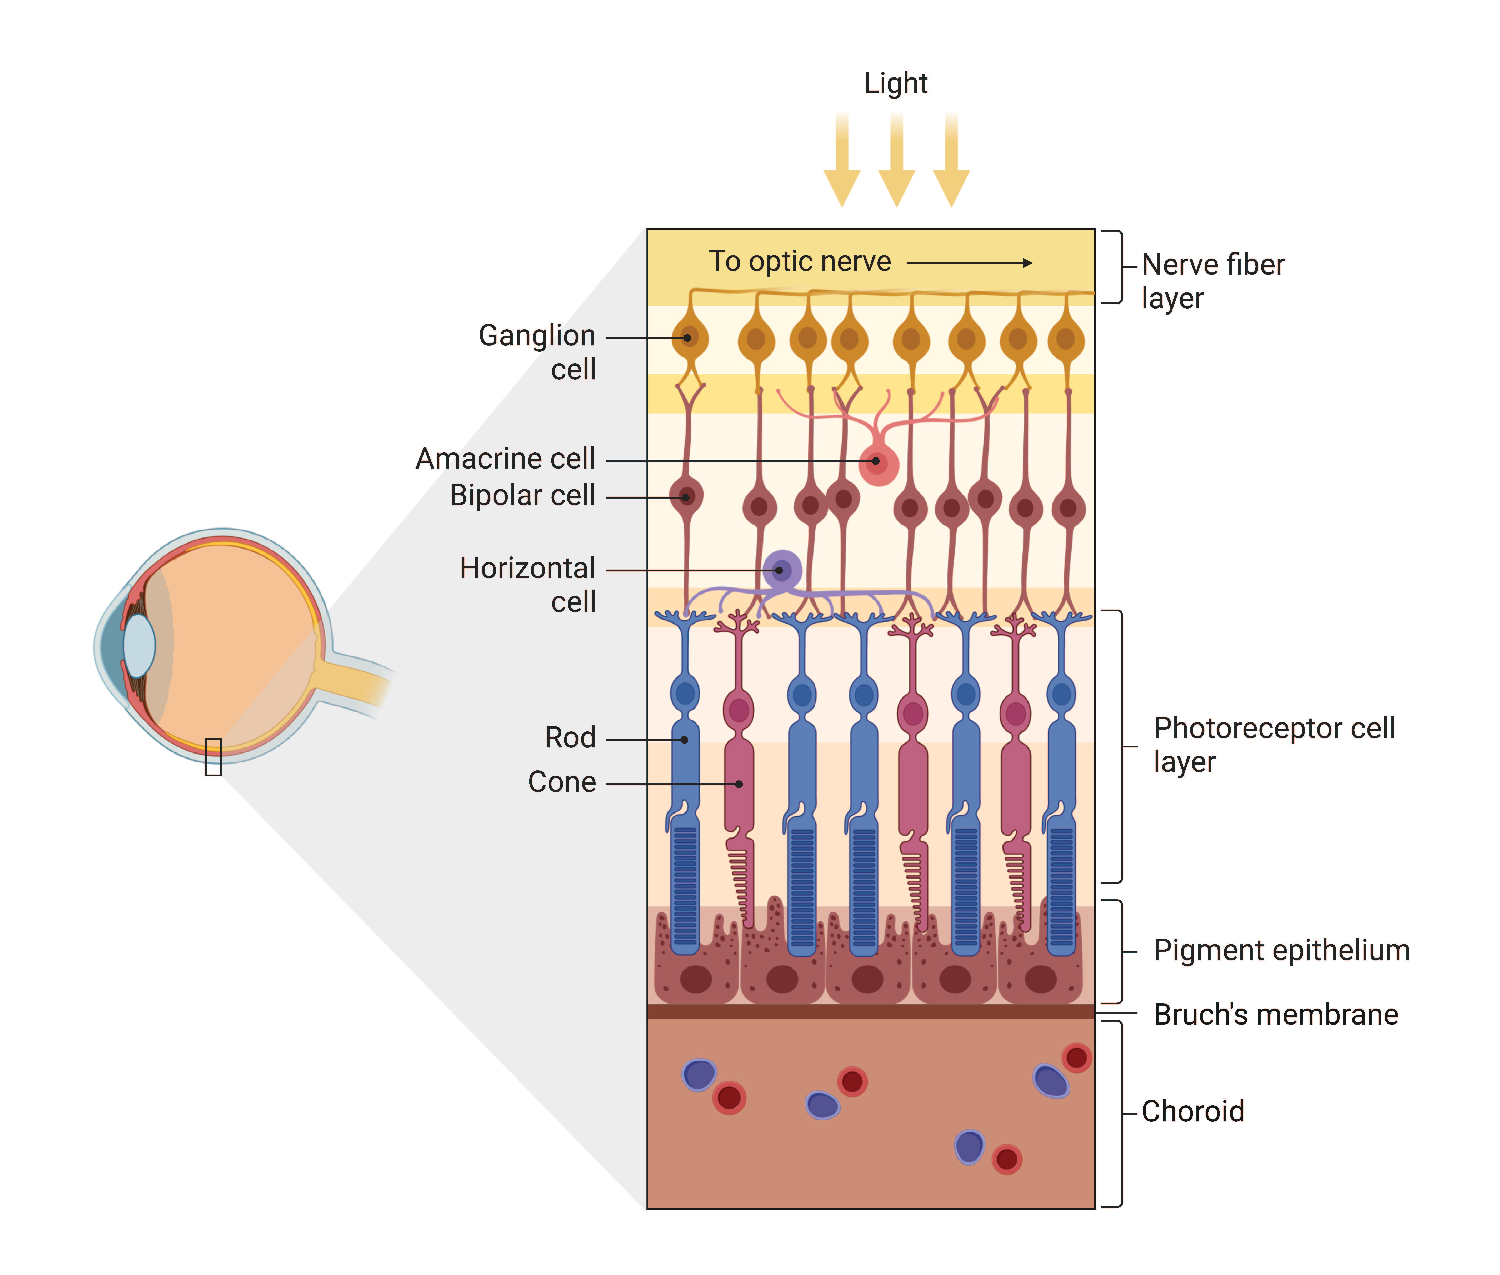
\includegraphics[width=\linewidth]{img/retina_anatomy.pdf}
    \caption{\textbf{A layered anatomy of retina} An illustration of a structural layers of a retina. Based on \citet{schwartz1991principles} (4th Edition), p. 436 and \citet{purves2019neurosciences} (6th Edition), p. 239. "Created in BioRender. Beinhauer, D. (2025) https://BioRender.com/oy5qz9v".}
    \label{fig:retina_anatomy}
\end{figure}

The first stage of visual processing occurs in photoreceptor cells,
which consist of \emph{rods} and \emph{cones}. These cells convert light into
chemical signals through photochemical reactions occurring in proteins within
their outer segments. Rods are highly sensitive to low light levels and detect
a broad spectrum of wavelengths, making them essential for night vision. 
In contrast, cones are selective for specific wavelengths and are less sensitive
to dim light, playing a key role in color vision and high-acuity visual perception. 
The distribution of rods and cones across the retina is non-uniform: \emph{fovea},
the central part of the retina, is densely packed with cones, while the periphery
contains a higher concentration of rods. Furthermore, there exists a \emph{blind spot} 
where the optic nerve exits the eye, without photoreceptors.    

Upon activation by light, photoreceptors undergo hyperpolarization, leading to a decrease
in the release of the neurotransmitter \emph{glutamate}. This neurotransmitter is then
detected by bipolar cells, which relays the processed signal to the next layer of the
retinal circuitry. In particular, unlike most neurons, all retinal cells except ganglion
cells do not generate action potentials but rather modulate their activity via graded potentials.

Bipolar cells, numbering approximately 10 million, integrate information from around
125 million photoreceptors. The number of photoreceptors connected to each bipolar
cell depends on the type of cell and the location of the retina. Horizontal cells contribute 
to this processing by integrating information from multiple photoreceptors and
providing contrast-enhancing feedback to bipolar cells.

Bipolar cells are categorized into two main types: \emph{ON bipolar cells} 
and \emph{OFF bipolar cells}. Their classification is based on how they 
respond to light. ON bipolar cells are activated in the presence of light, 
while OFF bipolar cells respond to darkness. These cells exhibit
\emph{center-surround receptive fields}, which means that they react positively to light
stimulation in the central region of their receptive field and negatively to
light in the surrounding region, an effect facilitated by horizontal cells. 
The size and sensitivity of the receptive fields vary depending on their location in the retina and the associated photoreceptors.

The final stage of retinal processing occurs in the ganglion cells, 
which work closely with amacrine cells. The signal processing mechanisms
in these cells follow similar center-surround organization principles as in
the bipolar and horizontal cells. Unlike other retinal neurons, ganglion
cells generate \emph{action potentials} due to their role in transmitting
visual information over long distances to the brain. Their axons form the
\emph{optic nerve}, which conveys the processed signal to the
\emph{Lateral Geniculate Nucleus} (LGN) of the thalamus, the next major relay
station on the visual pathway.

\section{Lateral Geniculate Nucleus}
\label{sec:lgn}
The next stage of visual processing occurs in the \emph{Lateral Geniculate Nucleus (LGN)}, 
a subcortical structure located within the thalamus. The LGN serves as the main relay center
for visual information, receiving input from retinal ganglion cells and
subsequently transmitting signals to primary visual cortex (V1) via optic radiation. 
Since V1 is the primary site of conscious visual perception, lesions along the pathway from the
retina through the LGN to V1 can result in varying degrees of visual impairment or blindness. 
The hierarchical organization of the visual system allows for precise localization of functional
deficits within specific neural structures.

Interestingly, a significant proportion of LGN input originates from V1 rather than from the retina. 
Although the exact function of these reciprocal cortico-thalamic connections remains an open question, 
they are thought to play a role in top-down modulation, facilitating attentional mechanisms
and gain control of sensory signals.

Structurally, the LGN is organized into six distinct layers, each receiving monocular input. 
These layers are further divided between the two eyes in a precise arrangement that maintains
the segregation of visual information from each eye. The receptive fields of LGN neurons exhibit a
concentric organization similar to retinal ganglion cells, with antagonistic properties surrounding the center.

\section{Primary Visual Cortex}
\label{sec:v1}
The primary visual cortex (V1), located in the occipital lobe, constitutes the first
cortical processing stage dedicated to visual analysis. It is responsible for extracting
fundamental features of the visual stimulus, including orientation, spatial frequency, 
motion, and color. Following initial processing, visual information is distributed into two main pathways: the parvocellular (P) pathway, which primarily involves
high-resolution spatial processing and object recognition, and the magnocellular (M) pathway, 
which specializes in motion detection and temporal dynamics.

V1 is organized into six histologically distinct layers, conventionally labeled with
Roman numerals. The primary input from the LGN is directed to layer IV, which is divided into four sublayers (IVA, IVB, IVC$\alpha$, and IVC$\beta$). Layer IVC, 
in particular, serves as the principal recipient of LGN projections, processing
monocular input before distributing signals to layers II and III, where binocular
integration occurs. From these layers, information is transmitted to higher-order 
visual areas such as V2, V3, and beyond, enabling progressively more complex visual
computations. Layers V and VI are primarily involved in feedback connections, 
modulating activity within earlier visual processing stages.

Intricate interlaminar connectivity is a hallmark of V1, particularly within layer IV, 
where excitatory and inhibitory neurons form recurrent circuits that refine feature
detection. Although inhibitory interneurons predominantly exert influence within their
respective layers, excitatory pyramidal neurons extend projections across multiple
layers, facilitating hierarchical processing.

A critical organizational feature of V1 is \emph{retinotopy}, where the spatial
arrangement of neurons preserves the topographical representation of the retina. 
However, this mapping is non-uniform, with a disproportionately large cortical
representation of the fovea relative to peripheral visual fields, reflecting the
greater density of photoreceptors in central vision.

\subsection{Receptive field properties of V1 cells}
\label{subsec:receptive_field}
V1 neurons exhibit selectivity for different stimulus attributes, forming
overlapping computational maps that encode various aspects of the visual scene. 
These selectivities include:

\begin{description}
    \item[Orientation selectivity:] Neurons in the layer IVC ($\alpha$ and $\beta$) begin to exhibit elongated receptive fields, departing from the concentric organization observed in earlier visual processing stages. This transformation enables sensitivity to the orientation of edges and lines, with each neuron preferentially responding to a specific angular configuration. The arrangement of orientation-selective neurons follows a columnar organization, in which cells with similar orientation preferences are clustered.
    \begin{description}
        \item[Simple Cells:] Simple cells demonstrate selectivity not only for orientation 
        but also for the precise spatial positioning of an edge within their receptive field. 
        Their response properties are derived from the summation of inputs from multiple LGN cells arranged antagonistically.
        \item[Complex Cells:] Complex cells, in contrast, maintain orientation selectivity but are less constrained by stimulus position within their receptive field. They 
        integrate signals from multiple simple cells, resulting in robust responses to oriented edges regardless of their exact location.
    \end{description}
    \item[Direction Selectivity:] Certain V1 neurons are tuned to the direction of motion, 
    responding preferentially to stimuli moving in a specific trajectory. These neurons play a crucial role in encoding motion dynamics and contribute to higher-order motion perception.
    \item[Binocularity:] While neurons in layer IV process monocular input primarily, subsequent layers integrate signals from both eyes, enabling binocular depth perception through mechanisms such as disparity tuning.
    \item[Additional Functional Specializations:] Beyond orientation and motion selectivity, 
    subsets of V1 neurons are specialized for processing stereoscopic depth, color opponency, 
    and feedback modulation from higher-order cortical areas.
\end{description}

\section{Extrastriate Visual Cortex}
\label{sec:extrastriate}
Beyond V1, visual processing continues in a network of extrastriate cortical regions
that extract increasingly abstract features of the visual scene. These areas include
V2, V3, V4, and MT (middle temporal area), each contributing to distinct aspects of
perception such as object recognition, motion tracking, and depth analysis. Damage
to these regions does not typically result in complete blindness, but instead leads to
specific deficits, such as achromatopsia (loss of color perception) or motion blindness
(inability to perceive fluid motion), depending on the affected region.
